\documentclass[12pt]{article}
\usepackage{cite}
\usepackage{graphicx}
\usepackage{subcaption}

\linespread{1.25} % the equivalent of 1.5 line spacing from msword
\usepackage[a4paper, left=2.5cm,right=2.5cm,top=2.5cm,bottom=2.5cm]{geometry} % margins


\title{Web service workload prediction using deep learning - Report 3}
\date{\today}
\author{Stefan Sebastian}

\begin{document}
  \maketitle
  \pagenumbering{gobble}
  \newpage 
  \pagenumbering{arabic}

  \section{State of the art}
  TODO 

  \section{Approach}
  The main goal is to find a performant model for web application 
  workload prediction, which can be later used by a proactive 
  microservice scaler. The methods used are different architectures
  of deep learning models: MLP, CNN, CNN-LSTM hybrid. The main 
  contribution of this research is the application of deep learning 
  to this specific problem and the comparison with a classic timeseries
  approach (ARIMA).

  The problem design has been influenced by the goal of integrating
  this model into a proactive microservice scaler. First of all,
  the choice of the workload measure is number of requests. The idea
  is that the scaling prediction should not influence the predicted 
  value, as would be the case with CPU or memory usage. Also this is 
  in line with research done by Jindal et al\cite{msc} who propose 
  a metric for measuring microservice performance based on number of 
  satisfied requests. Another consideration is the prediction interval.
  Taking into account the experience of Netflix\cite{scryer}, who run 
  a microservice architecture in production, the time window should be in 
  the order of minutes, so you can predict spikes and have time to deploy
  new service instances.

  A realistic workload has been used for this experiment, a wikipedia 
  trace for 12 days in september 2007. From this a subset of requests was 
  extracted (all requests for Japanese wikipedia). The subset was selected 
  in order to compare results with Kim et al.\cite{CloudInsight} which used 
  the same dataset. In order to turn a web request log file into a supervised 
  dataset the following steps were taken: create buckets which contain the 
  number of requests in a time interval, iterate over the buckets using 
  the sliding window technique\cite{sliding_window}. Basically we generate 
  training instances with input (t, t-1, ... t-n) and output (t+2). The 
  predicted value is t+2 instead of t+1 because a scaler using this model 
  would need to have a buffer window during which to deploy the services.

  After preparing the dataset two baseline models were prepared: the naive 
  approach (predict traffic in window t+2 to be traffic in t) and a classic 
  timeseries model (ARIMA). The next step was to experiment with different 
  deep learning architectures and measure the results.


  \section{Evaluation of the approach}
  \subsection{Validation and tuning}
  Model tuning and validation was done on the Japanese wikipedia trace because 
  although presenting some patterns it also has some interesting irregularities, 
  like a huge spike which is not repeated. The selected time window for tuning 
  is 10 min. (todo test on other windows - tune on other windows?)

  The dataset is split into a training and testing with a ratio of 0.9.
  The validation method is k-fold Cross-Validation\cite{kfold} with k = 3, 
  which means splitting the training dataset into k equal parts, perform training
  on k - 1 and evaluation on the part left out. This process is repeated k times.
  The main idea is to not touch the testing data while tuning the model, so the 
  model will not be influenced by it.

  \subsection{Performance metrics}
  TODO detail mse, mape, mae

  \subsubsection{Naive baseline}
  A naive baseline is set, to get an idea if the models are useful at all. The 
  naive predictor simply states that traffic in window t+2 will be the same as 
  in the last measured window. The prediction is ploted in figure \ref{fig:baseline_pred}
  and achieves MSE: 20234787.901, MAE: 3572.657, MAPE: 7.072.


  \begin{figure}
    \centering
    \begin{subfigure}[b]{0.48\linewidth}
      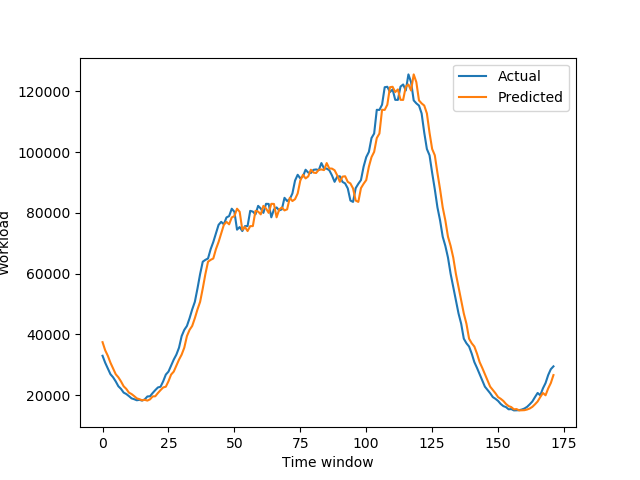
\includegraphics[width=\linewidth]{resources/baseline/naive_predictions_10.png}
      \caption{Naive prediction}
    \end{subfigure}
    \begin{subfigure}[b]{0.48\linewidth}
      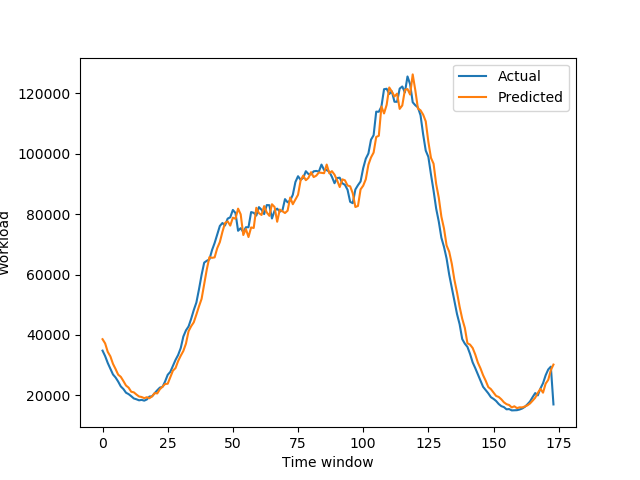
\includegraphics[width=\linewidth]{resources/baseline/arima_10.png}
      \caption{Arima prediction}
    \end{subfigure}
    \caption{Baseline predictions}
    \label{fig:baseline_pred}
  \end{figure}

  \subsubsection{ARIMA}
  ARIMA\cite{arima}, which stands for autoregressive integrated moving average, is a classic approach 
  to modelling timeseries. In order to apply this model we need to find appropiate values for its 
  parameters: p, q, d. 
  
  The value of d means the number of times the series needs to be differentiated
  in order to make it stationary. The series stationarity was checked using the augmented Dickey-Fuller 
  test\cite{Dickey-Fuller} which found the p-value to be 1.0902496274664773e-08. This is lower than 0.05, 
  the commonly used threshold, meaning we can set d to 0. 
  
  The partial autocorrelation plot was analyzed
  to set the autoregression parameter (p). From figure \ref{fig:arima_params} we can see that the significance
  region is confidently passed at 1, with a steep decline afterwards. The moving average parameter (q) is 
  approximated from the autocorrelation plot. It suggests a value of around 20 would be a good start. 
  After fitting ARIMA(1,0,20) the final 2 layers had P-value of 0.547 and 0.758 which meant that they were 
  not significant. After trying some values for q: 5,10,15,18 the best results were obtained on ARIMA(1,0,15)
  with MSE: 15289199.210, MAE: 3118.982, MAPE: 6.782.

  \begin{figure}
    \centering
    \begin{subfigure}[b]{0.4\linewidth}
      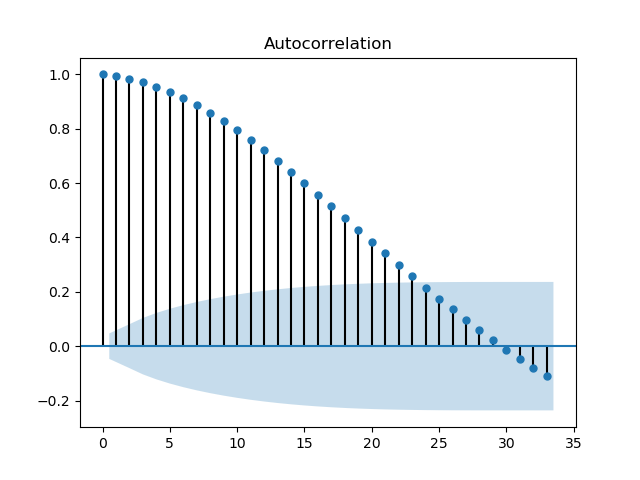
\includegraphics[width=\linewidth]{resources/baseline/arima_10_acf.png}
      \caption{Autocorrelation plot}
    \end{subfigure}
    \begin{subfigure}[b]{0.4\linewidth}
      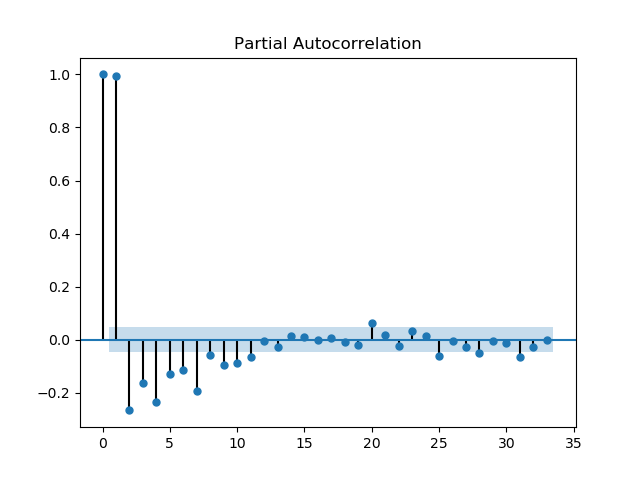
\includegraphics[width=\linewidth]{resources/baseline/arima_10_pacf.png}
      \caption{Partial autocorrelation plot}
    \end{subfigure}
    \caption{ARIMA params}
    \label{fig:arima_params}
  \end{figure}


  \newpage
  \bibliography{bibliography}{}
  \bibliographystyle{plain}
\end{document}